\spis{Od mnożenia do dodawania}
{Michał Miśkiewicz}


\newcommand{\dlink}[3]{\href{#1}{$\Delta^{#2}\sb{#3}$}}

\label{Od mnozenia do dodawania}
\wtyt{Od mnożenia\\ do dodawania}
\waut{Michał MIŚKIEWICZ*}
\aafil{Wydział Matematyki, Informatyki i~Mechaniki, Uniwersytet Warszawski}
\marg{Źródło: Carl B. Boyer, \emph{A~history of mathematics}, 2nd edition, 1991. Interesująca nas historia jest na str.~307--315.}

\vspace{-25mm}
\epigraph{
\emph{Don't know much about geography \\
Don't know much trigonometry \\
Don't know much about algebra \\
Don't know what a~slide rule is for}\vspace*{-3pt}
}{``Wonderful world'', Sam Cooke\vrule height10pt width0pt} 
\vspace{-2mm}
%\end{szeroko}

Od powstania piosenki Sama Cooke'a minęły 64 lata. Wśród dziedzin wiedzy, które jej bohater wymienia jako swoje słabe strony, jedna w~międzyczasie wypadła z~programów nauczania. 
Mianowicie, młodszy Czytelnik ma pełne prawo nie wiedzieć, do czego służy suwak logarytmiczny (\emph{slide rule}). Warto ten stan zmienić. W~\emph{Delcie} można już było o~suwaku przeczytać w~\dlink{https://deltami.edu.pl/1981/08/suwak-logarytmiczny-komputer-xvii-wieku/}{8}{81} i~\dlink{https://deltami.edu.pl/2001/12/zrob-sobie-suwak-logarytmiczny/}{12}{01}, ale myślę, że i~tak warto powiedzieć kilka słów o~idei jego działania wraz z~historycznym kontekstem. 
%Jako że o samym suwaku można już było w \emph{Delcie} przeczytać \red{(gdzie dokładnie?)}, tutaj więc skupię się na idei jego działania wraz z historycznym kontekstem. 
%Żeby skupić się na sednie problemu, pozwoliłem sobie na pewne historyczne przekłamania

Do czego zatem służy suwak logarytmiczny? 
\marg{
Poniższy żart pokazuje, że mnożenie może się okazać trudniejsze od dodawania. \\[1mm]
\emph{Noah sent his animals to ``go forth and multiply'', but a~pair of snakes told him ``we can't multiply, we're adders!''.
}\bigskip}
%Najprostsza odpowiedź brzmi: 
Otóż do tego, by zamiast działania mnożenia można było wykonywać dodawanie. No dobrze, a~dlaczego miałoby nam na tym zależeć (pomijając żarty o~rozmnażaniu żmij)? Jako odpowiedź przytoczmy szkolne ,,działania pod kreską'', dla przykładu przedstawione na marginesie dla liczb $1{,}284$ i $2{,}117$. 
\marg{
\begin{center}
\begin{tabular}{@{}c*{4}{@{\,}c}@{}}
  & 1{,} & 2 & 8 & 4 \\
+ & 2{,} & 1 & 1 & 7 \\
\hline 
\vrule height8pt width0pt  & 3{,} & 4 & 0 & 1 
\end{tabular}
\hspace{5mm}
%\begin{tabular}{l*{7}{@{\,}l}}
\begin{tabular}{@{}c@{\,}l@{}l@{\,}l@{\,}l@{}l@{\,}l@{\,}l@{}}
& & & 	   & 1{,} & 2 & 8 & 4 \\
& & $\times$\hspace{-1mm} & & 2{,} & 1 & 1 & 7 \\
\hline 
\vrule height8pt width0pt	&      &   &   & 8 & 9 & 8 & 8 \\
	& 	   &   & 1 & 2 & 8 & 4 & \\
	& 	   & 1 & 2 & 8 & 4 &   & \\
$+$ & 2    & 5 & 6 & 8 &   &   & \\
\hline
\vrule height8pt width0pt    & 2{,} & 7 & 1 & 8 & 2 & 2 & 8
\end{tabular}
% MM: to jest najprostszy sposób na wyświetlenie tego, ale nie ma się wtedy wpływ na wygląd
%\opmul{1.284}{2.117}
\end{center}
Rys. 1. Dodawanie i~mnożenie ,,pod kreską'' liczb $1{,}284$ i $2{,}117$. Drugi z~algorytmów ma zauważalnie większą złożoność 
}
Widać, że mnożenie jest dużo bardziej pracochłonne: dla dwóch liczb $n$-cyfrowych znalezienie sumy wymaga około $n$~operacji, a~iloczynu -- około~$n^2$. 

\styt{Jak mnożyć, dodając?} 
Ta trudność dała się we znaki astronomom XVI wieku ze względu na ilość i~dokładność obliczeń koniecznych w~ich pracy. Dla jej pokonania opracowali metodę o~nazwie \emph{prosthaphaeresis}, od greckich słów oznaczających dodawanie i~odejmowanie. Opierała się na tożsamościach trygonometrycznych, takich jak 
\[
\cos \alpha \cdot \cos \beta 
= \left( \cos(\alpha+\beta) + \cos(\alpha-\beta) \right) / 2,
\]
\marg{
Oprócz wzoru na iloczyn cosinusów %(i~podobnych wzorów trygonometrycznych) 
zamianie mnożenia na prostsze operacje może służyć tożsamość $xy = ((x+y)^2 - (x-y)^2)/4$. Oparta na niej metoda (\emph{quarter square multiplication}) stała się jednak popularna dopiero dużo później.
Znając stosunek bohatera piosenki do trygonometrii i~algebry, można mieć niemal pewność, że nie byłby on zadowolony z~żadnego z~tych wzorów. 
%Wzór na iloczyn cosinusów znał już ibn~Yunus (ok. 950--1009), przypisuje się go też Johannesowi Wernerowi (1468--1522), jednak dopiero pod koniec XVI wieku astronomowie (m.in. Tycho Brache i~Christoph~Clavius) zaczęli go wykorzystywać do mnożenia liczb. 
%Bohater piosenki najpewniej tego wzoru nie znał. 
}oraz na użyciu tablic trygonometrycznych. Tablice takie dobrze znają maturzyści, ponieważ w~trakcie egzaminu mogą odczytywać z~nich wartości funkcji $\sin$, $\cos$, $\tan$ dla wielokrotności $1^\circ$; w~XVI wieku były jednak w~użyciu tablice dużo dokładniejsze (np. co do sekundy kątowej). A~metoda wygląda następująco: 
\begin{enumerate}[nosep]
\item Odnajdujemy w~tablicy nasze czynniki jako wartości cosinusa. Ze zrozumiałych względów nie znajdziemy tam $1{,}284$ i $2{,}117$, ale $0{,}1284$ i $0{,}2117$ już tak -- odpowiadają one w~przybliżeniu kątom $\alpha = 82{,}623^\circ$ i $\beta = 77{,}778^\circ$. 
\item Wykonujemy dodawanie i~odejmowanie (stąd wzięła się nazwa metody): $\alpha + \beta = 160{,}401^\circ$, $\alpha - \beta = 4{,}845^\circ$. 
\item Odczytujemy przybliżone wartości cosinusa tych kątów: $\cos(\alpha + \beta) = -0{,}94206$, $\cos(\alpha-\beta) = 0{,}99643$, a~na koniec bierzemy średnią: $0{,}027185$. Ostateczny wynik wymaga jeszcze przesunięcia przecinka: $2{,}7185$. 
\end{enumerate}
Otrzymaliśmy w~ten sposób $1{,}284 \cdot 2{,}117 \approx 2{,}7185$, co może nie zachwyca, ale oczywiście dokładność obliczeń można dowolnie zwiększać, sięgając po coraz lepsze tablice. 
% Tablice maturalne jako wynik mnożenia 1.284*2.117 dają wynik 2.74 zamiast 2.718228 (po drodze trzeba przesunąć przecinek)

Niedługo później wymyślono tablice logarytmiczne, 
\marg{
\begin{tabular}{@{}c*{11}{@{\,\,}c}@{}}
0 & 1 & 2 & 3 & 4 & 5 & 6 & 7 & 8 & 9 & 10 & 11 \\
\hline
\vrule height8pt width0pt 1 & 2 & 4 & 8 & 16 & 32 & 64 & 128 & 256 & 512 & 1024 & 2048
\end{tabular} \\[2mm]
Rys. 2. Przodek tablic logarytmicznych: tablica kolejnych potęg dwójki. Podobne ciągi są obecne w~pracach Archimedesa, były też regularnie publikowane w~XVI wieku, np. w~\emph{Arithmetica integra} Michaela Stifela (1544)
}
niejako szyte na miarę rozważanego przez nas problemu. Jako bezpośredniego przodka takich tablic możemy wskazać tablicę potęg dwójki (na marginesie). Umożliwia ona szybkie mnożenie liczb z~drugiego wiersza tablicy. 
Przykładowo, iloczyn $32$ i $64$ moglibyśmy wyznaczyć pod kreską, możemy też jednak odczytać z~tablicy, że są to potęgi $2^5$ i $2^6$, dają więc po wymnożeniu $2^{11} = 2048$. Ponownie udało nam się oszukać przeznaczenie i~dodać zamiast pomnożyć. Opisana metoda ma jednak oczywistą podstawową wadę: liczby w~drugim rzędzie tablicy nie są równo rozmieszczone na prostej, a~im dalej, tym odległości między nimi większe. W~rezultacie metoda jest mało praktyczna, bo w~typowej sytuacji nie znajdziemy w~drugim rzędzie interesujących nas czynników, nawet w~przybliżeniu. 

\styt{Krótka historia logarytmu.} 
Problem ten rozwiązali niezależnie John Napier (1550--1617) i~Jost B\"urgi (1552--1632), jednak ze względu na pierwszeństwo publikacji (1614 vs. 1620) to ten pierwszy wpłynął na dalsze losy matematyki. Pomysł jest prosty: aby liczby z~drugiego wiersza były gęściej (i~równiej) rozmieszczone, należy jako podstawę wziąć liczbę bliższą jedynki, na przykład $1{,}0001$. Podnosząc tę liczbę do kolejnych potęg, otrzymujemy dość długą tablicę, której część jest przedstawiona na marginesie. Interesujące nas liczby odnajdujemy w~sensownym przybliżeniu na pozycjach 2500 i~7500, co po dodaniu daje 10 000, więc jako przybliżony iloczyn odczytujemy $2{,}71815$. Tak jak dla prosthaphaeresis, tak i~tutaj dokładność można dowolnie zwiększać. Poraża za to prostota samej procedury -- nic dziwnego, że pomysł Napiera upowszechnił się jeszcze przed publikacją B\"urgiego. Niedługo później, gdzieś pomiędzy rokiem 1620 a~1630, wymyślono \emph{suwak logarytmiczny}, poręczne narzędzie oparte na tablicy logarytmicznej. Ale o~tym potem. 
\marg{
% log(1.284)/log(1.0001) = 2399.927... 
% log(2.117)/log(1.0001) = 7500.375...
\begin{center}
\begin{tabular}{@{}r|l@{}}
%$\log_{1{,}0001}(x)$ & $x$ \\
$n$ & $1{,}0001^n$ \\
\hline
\vrule height8pt width0pt0  &  1,0000 \\
1  &  1,0010 \\
2  &  1,0020 \\
3  &  1,0030 \\
\ldots & \ldots \\
2499  &  1,28388 \\
2500  &  \textbf{1,28401} \\
2501  &  1,28414 \\
\ldots & \ldots \\
7499  &  2,11671 \\
7500  &  \textbf{2,11692} \\
7501  &  2,11713 \\
\ldots & \ldots \\
9999   &  2,71787 \\
10000  &  \textbf{2,71815} \\
10001  &  2,71842 
\end{tabular}
\end{center}
Rys. 3. Tablica logarytmiczna podobna do oryginalnej tablicy B\"urgiego. Napier jako podstawę przyjął $1-10^{-7}$, a~więc liczbę mniejszą od jedynki 
}

Wróćmy na chwilę do zagadnienia większej dokładności. Jeśli w~którymś miejscu po prawej stronie widzimy liczbę $x$, to liczbę po lewej nazywamy \emph{logarytmem} z $x$ o~podstawie $1{,}0001$, co zapisujemy jako $\log_{1{,}0001}(x)$ -- ponownie nazwa pochodzi od dwóch greckich słów, tym razem oznaczających stosunek (\emph{logos}) i~liczbę (\emph{arithmos}). Wynik w~oczywisty sposób zależy od przyjętej podstawy, i~tę zależność łatwo prześledzić, próbując podstaw postaci $1+10^{-k}$ dla kolejnych naturalnych $k$. Okazuje się, że przy zwiększaniu $k$ liczba $\log_{1+10^{-k}}(x)$ z~grubsza wydłuża się o~kolejne zera. Gdybyśmy chcieli móc zestawiać tablice o~różnej dokładności, to warto umówić się, że wszystkie liczby w~lewej kolumnie podzielimy przez $10^k$, czyli obok $x$ wpiszemy liczbę $10^{-k} \log_{1+10^{-k}}(x)$. Dla dużych~$k$ tak określona funkcja przybliża tak zwany \emph{logarytm naturalny}, oznaczany przez $\ln(x)$. Jest to logarytm o~podstawie $e \approx 2{,}71828$. Liczba $e$ nazywana jest liczbą Eulera lub Napiera, albo też -- podstawą logarytmu naturalnego! 

Warto tu napomknąć, 
\marg{
We współczesnym języku kinematyczny opis Napiera sprowadza się do równań różniczkowych 
\[
\begin{cases}
\dfrac{dx}{dt} = -x\smallskip \\
x(0) = 1,
\end{cases}
\begin{cases}
\dfrac{dy}{dt} = 1 \smallskip\\
y(0) = 0.
\end{cases}
\]
%$\frac{dx}{dt} = x$ i $\frac{dy}{dt} = 1$. 
Otrzymujemy z~nich $\frac{dy}{dx} = -\frac 1x$, a~więc po uwzględnieniu warunków początkowych $y(x) = -\ln(x)$. 
}
że ów \emph{naturalny} logarytm pochodzi od samego Napiera. 
%że sam Napier był świadomy istnienia owego \emph{naturalnego} logarytmu. 
Chociaż swoją tablicę wyznaczył on poprzez potęgowanie konkretnej liczby bliskiej jedynce, to jako definicję logarytmu podał następujący opis kinematyczny, poniżej nieco tylko uwspółcześniony. W~chwili $t = 0$ punkty $x$, $y$ na osi liczbowej są odpowiednio w $1$, $0$ oraz mają prędkość jednostkową -- $x$ w~lewo, a $y$ w~prawo. Przy tym prędkość $y$ jest stała, a~prędkość $x$ jest proporcjonalna do odległości od zera. Jako logarytm z $x(t)$ definiujemy wtedy $-y(t)$.

Z~opisu tego rzeczywiście wynika, że $y$ jest logarytmem naturalnym z $x$ (z~minusem). Podnoszenie $1-10^{-7}$ do kolejnych potęg -- to właśnie robił Napier -- odpowiada dyskretyzacji problemu, czyli przyjęciu, że prędkość $x(t)$ zmienia się skokowo w~odstępach czasowych $\Delta t = 10^{-7}$. Zastosowanie dyskretyzacji sugeruje, że Napier był świadomy zbieżności przy $\Delta t \to 0$, co równoważne jest zbieżności $(1 + \frac 1n)^n \to e$ przypisywanej\dots\ Eulerowi. 

\styt{Dygresja o~teorii Eulera.}
%\styt{Eulera teoria wszystkiego.} 
Obecnie typowy wykład analizy matematycznej nie odzwierciedla historycznego rozwoju tej dziedziny, a~zamiast tego referuje dokonania Leonharda Eulera (1707--1783). Wprowadził on funkcję wykładniczą zadaną szeregiem 
\begin{equation}
\label{eq:def-exp}
\tag{$\star$}
e^x = 1 + \frac{x}{1!} + \frac{x^2}{2!} + \frac{x^3}{3!} + \frac{x^4}{4!} + \ldots
\end{equation}
lub równoważnie jako granicę $\left( 1+\frac{x}{n} \right)^n$ przy $n \to \infty$. Dowiódł, że jest to funkcja odwrotna do logarytmu naturalnego, czyli spełnione są równości $e^{\ln(x)} = x$ (dla $x > 0$) i $\ln(e^y) = y$ (dla $y \in \mathbb R$). W~szczególności $e^1$ to dokładnie $e$, natomiast $e^n$ jest równe 
$n$-krotnemu iloczynowi $e \cdot \ldots \cdot e$, i~ogólnie zachodzi wzór $e^x \cdot e^y = e^{x+y}$. 
%$\underbrace{e \cdot \ldots \cdot e}_{n \text{ razy}}$ 
Nie należy jednak dać się zmylić: 
\marg{
We wzorze \eqref{eq:def-exp} za liczbę $x$ można przyjąć dowolną liczbę zespoloną, a~tożsamość $e^x \cdot e^y = e^{x+y}$ (tzw. prawo grupowe) nadal pozostaje w~mocy. Funkcję cosinus można zdefiniować (i~tak się zazwyczaj robi!) jako $\cos(x) := (e^{ix}+e^{-ix})/2$. Wzór na iloczyn cosinusów nie jest wtedy twierdzeniem geometrycznym, ale banalną konsekwencją prawa grupowego: obie strony okazują się równe $\frac 14 (e^{ix+iy} + e^{-ix-iy} + e^{ix-iy} + e^{-ix+iy})$.
%\begin{gather*}
%\cos(x) \cdot \cos(y) \\
%= \frac{e^{ix+iy} + e^{-ix-iy} + e^{ix-iy} + e^{-ix+iy}}{4} \\
%% = (\cos(x+y) + \cos(x-y))/2.
%\end{gather*}
}
liczby takie jak $e^{\sqrt{2}}$ nie wymagają od nas $\sqrt{2}$-krotnego mnożenia, a~jedynie podstawienia $x = \sqrt{2}$ do nieskończonej sumy~\eqref{eq:def-exp}. Funkcja $e^x$ to zatem coś więcej niż potęgowanie. Ta uwaga niesie ze sobą wiele pożytecznych konsekwencji, między innymi pozwala wyjaśnić rzecz następującą. Czy zdziwiło wcześniej Czytelnika, że funkcja $\cos$ podobnie jak $\ln$ ,,zamienia mnożenie na dodawanie''? Otóż obie te funkcje są spokrewnione z~funkcją $e^x$, co wyjaśnia ich magiczne własności -- szersze wyjaśnienie na marginesie. 



%\begin{szeroko}
\styt{Powrót do suwaka.} 
Zestawiając razem dwie zwyczajne linijki, otrzymujemy prosty przyrząd do dodawania. By dodać na nim liczby $3$ i $1$, przesuwamy linijki tak, by trójka pojawiła się nad zerem, a~wówczas wynik odczytujemy powyżej jedynki. Zgodnie z~oczekiwaniami, wyszło $4$. Ale spójrzmy na małą modyfikację:
\vskip\parskip

%\begin{center}
\rightline{\input{mm/rys-suwak-add}
\hspace{1mm}
\begin{tikzpicture}[x=4cm, y=4cm, every node/.style={font=\scriptsize}]
\draw[very thick] (-0.1,0) rectangle (1.1,0.2);
\foreach \i in {0, 1, 2}
	\draw (\i*0.25,0) -- ++(0,0.08) node[above] {$2^{\i}$};
\foreach \i in {3, 4}
	\draw[magenta, very thick] (\i*0.25,0) -- ++(0,0.08) node[above] {$2^{\i}$};
% dolna linijka
\begin{scope}[shift={(0.75,0)}]
\draw[very thick] (-0.1,0) rectangle (1.1,-0.2);
\foreach \i in {0, 2, 3, 4}
	\draw (\i*0.25,0) -- ++(0,-0.08) node[below] {$2^{\i}$};
\foreach \i in {1}
	\draw[magenta, very thick] (\i*0.25,0) -- ++(0,-0.08) node[below] {$2^{\i}$};
\end{scope}
\end{tikzpicture}}
%\end{center}

Pod każdą etykietą na obu linijkach dopisaliśmy dwójkę, w~ten sposób podmieniając ciąg arytmetyczny $0,1,2,\ldots$ na ciąg geometryczny $2^0,2^1,2^2,\ldots$ Tak jak w~przypadku rysunku~2, dodawanie zamieniło się na mnożenie potęg dwójki, u~nas konkretnie: $8 \cdot 2 = 16$. Ta modyfikacja to właśnie \emph{suwak logarytmiczny}. Oczywiście standardowy suwak dla wygody użytkowania uwzględnia na swojej skali takie liczby, jak $1,2,3,\ldots$, a~nie tylko potęgi dwójki. W~tym kontekście naturalne jest pytanie: \emph{a~gdzie te liczby umieścić?}, na które odpowiedzią jest właśnie logarytm: liczba $y$ pojawia się w~odległości $\log(y)$ od początku linijki (wybór podstawy logarytmu jest tu drugorzędny). Poniżej widać, jak można za pomocą takiego przyrządu pomnożyć liczby $e^{1/4} \approx 1{,}284$ i $e^{3/4} \approx 2{,}117$: 

%Weźmy zwyczajną linijkę i podmieńmy pojawiające się na niej liczby: w miejsce $x$ wpiszmy $e^x$ (wybór $e$ jako podstawy jest uświęcony zwyczajem, ale nieistotny; $2$ też zadziała). Powstała skala nosi nazwę \emph{logarytmicznej}, bo liczba $y$ pojawia się na niej w odległości $\ln(y)$ od początku linijki. Żeby uzyskać większą czytelność, warto umieścić podpisy w innych miejscach, by na skali pojawiały się liczby $1,2,3,\ldots$ zamiast $1,e,e^2,\ldots$, ale nie jest to kluczowe dla działania suwaka. A sam suwak otrzymujemy, zestawiając razem dwie linijki o~skali logarytmicznej. Poniżej widać, jak za pomocą takiego przyrządu pomnożyć liczby $e^{1/4} \approx 1{,}284$ i $e^{3/4} \approx 2{,}117$: 
%\red{(być może warto przygotować dwie wersje: jedną z ordynarną podziałką, a drugą z podziałką jak na prawdziwym suwaku)}

%\marg{Rys. 4. Jeśli linijki są tak przesunięte, by $e^a$ było bezpośrednio nad $e^0$, to $e^{a+b}$ jest nad $e^b$. \\[1mm]
%Drugi suwak różni się od pierwszego jedynie wyborem liczb zaznaczonych na skali, ale zasada działania jest ta sama: by pomnożyć liczby $x$ i $y$, przesuwamy $x$ nad $1$, a wynik $x \cdot y$ odczytujemy powyżej $y$. 
%}

%\marg{Rys. 4. Dwa suwaki logarytmiczne, różniące się jedynie wyborem liczb zaznaczonych na skali. W obu przypadkach zasada działania jest ta sama: jeśli chcemy pomnożyć liczby $x$ i $y$, to zestawiamy $x$ na górze z $1$ na dole, a wówczas $x \cdot y$ odczytujemy na górze, naprzeciwko $y$. 
%Obok przedstawiono mnożenie $e^{3/4} \cdot e^{1/4} = e$.
%}
%Suwak logarytmiczny, czyli dwie linijki A i B ze skalą logarytmiczną. Jeśli zestawimy $x$ na A z $1$ na B, to $x \cdot y$ na A jest naprzeciwko $y$ na B. Dwa suwaki obok różnią się jedynie wyborem liczb zaznaczonych na skali -- w pierwszym przypadku zasada działania jest bardziej naoczna.

%\begin{szeroko}
\begin{center}
%\input{rys-suwak-simple}
%\vspace{2mm}

\tikzstyle{sArrow}=[-{Stealth[length=2mm]}]
\scalebox{1.2}{\begin{tikzpicture}[x=4cm, y=4cm, every node/.style={font=\scriptsize}]
\draw[very thick] (-0.1,0) rectangle ({0.1+ln(4)},0.42);
%\draw[very thick] (-0.1,0) rectangle ({0.1+ln(4)},0.45);
\foreach \i in {1,2,3}
{
	% główna kreska
	\draw let \n1={ln(\i)} in
		(\n1,0) -- ++(0,0.12) node[above] {$\i$};
	% kreska w połowie
	\draw let \n1={ln(\i+0.5)} in
		(\n1,0) -- ++(0,0.11) node[above, scale=0.8] {$\i{,}5$};
	% dwie dodatkowe kreski
	\draw let \n1={ln(\i+0.25)} in
		(\n1,0) -- ++(0,0.05) node[above, scale=0.8] {$\i{,}25$};
	\draw let \n1={ln(\i+0.75)} in
		(\n1,0) -- ++(0,0.05) node[above, scale=0.8] {$\i{,}75$};
}
% ostatnia kreska
\draw let \n1={ln(4)} in
	(\n1,0) -- ++(0,0.12) node[above] {$4$};
% kreski na potrzeby obliczeń 
\draw[sArrow, magenta, thick] 
	(0.75,0.2) node[above] {$e^{3/4} \approx 2{,}117$} -- (0.75,0.02);
\draw[sArrow, magenta, thick] 
	(1.00,0.3) node[above] {$e \approx 2{,}718$} -- (1.00,0.02);

% dolna linijka
\begin{scope}[shift={(0.75,0)}]
\draw[very thick] (-0.1,0) rectangle ({0.1+ln(4)},-0.33);
%\draw[very thick] (-0.1,0) rectangle ({0.1+ln(4)},-0.45);
\foreach \i in {1,2,3}
{
	% główna kreska
	\draw let \n1={ln(\i)} in
		(\n1,0) -- ++(0,-0.12) node[below] {$\i$};
	% kreska w połowie
	\draw let \n1={ln(\i+0.5)} in
		(\n1,0) -- ++(0,-0.11) node[below, scale=0.8] {$\i{,}5$};
	% dwie dodatkowe kreski
	\draw let \n1={ln(\i+0.25)} in
		(\n1,0) -- ++(0,-0.05) node[below, scale=0.8] {$\i{,}25$};
	\draw let \n1={ln(\i+0.75)} in
		(\n1,0) -- ++(0,-0.05) node[below, scale=0.8] {$\i{,}75$};
}
% ostatnia kreska
\draw let \n1={ln(4)} in
	(\n1,0) -- ++(0,-0.12) node[below] {$4$};
% kreska na potrzeby obliczeń 
%\draw[magenta, very thick] (0.25,0) -- ++(0,-0.2) node[below] {$e^{1/4} \approx 1{,}284$};
\draw[sArrow, magenta, thick] 
	(0.25,-0.2) node[below] {$e^{1/4} \approx 1{,}284$} -- (0.25,-0.02);
\end{scope}
\end{tikzpicture}}
\end{center}
%\end{szeroko}

Bohater piosenki Sama Cooke'a miał silne, choć trudne do wyrażenia w~słowach przekonanie, że umiejętność dodawania jest wystarczająca. Wystarczająca nie tylko do tego, by mnożyć, ale też by spełnić marzenie o~odwzajemnionej miłości. Lubię więc myśleć, że co nieco jednak wiedział o~naturze suwaka logarytmicznego. Posłuchajmy sami:\marg{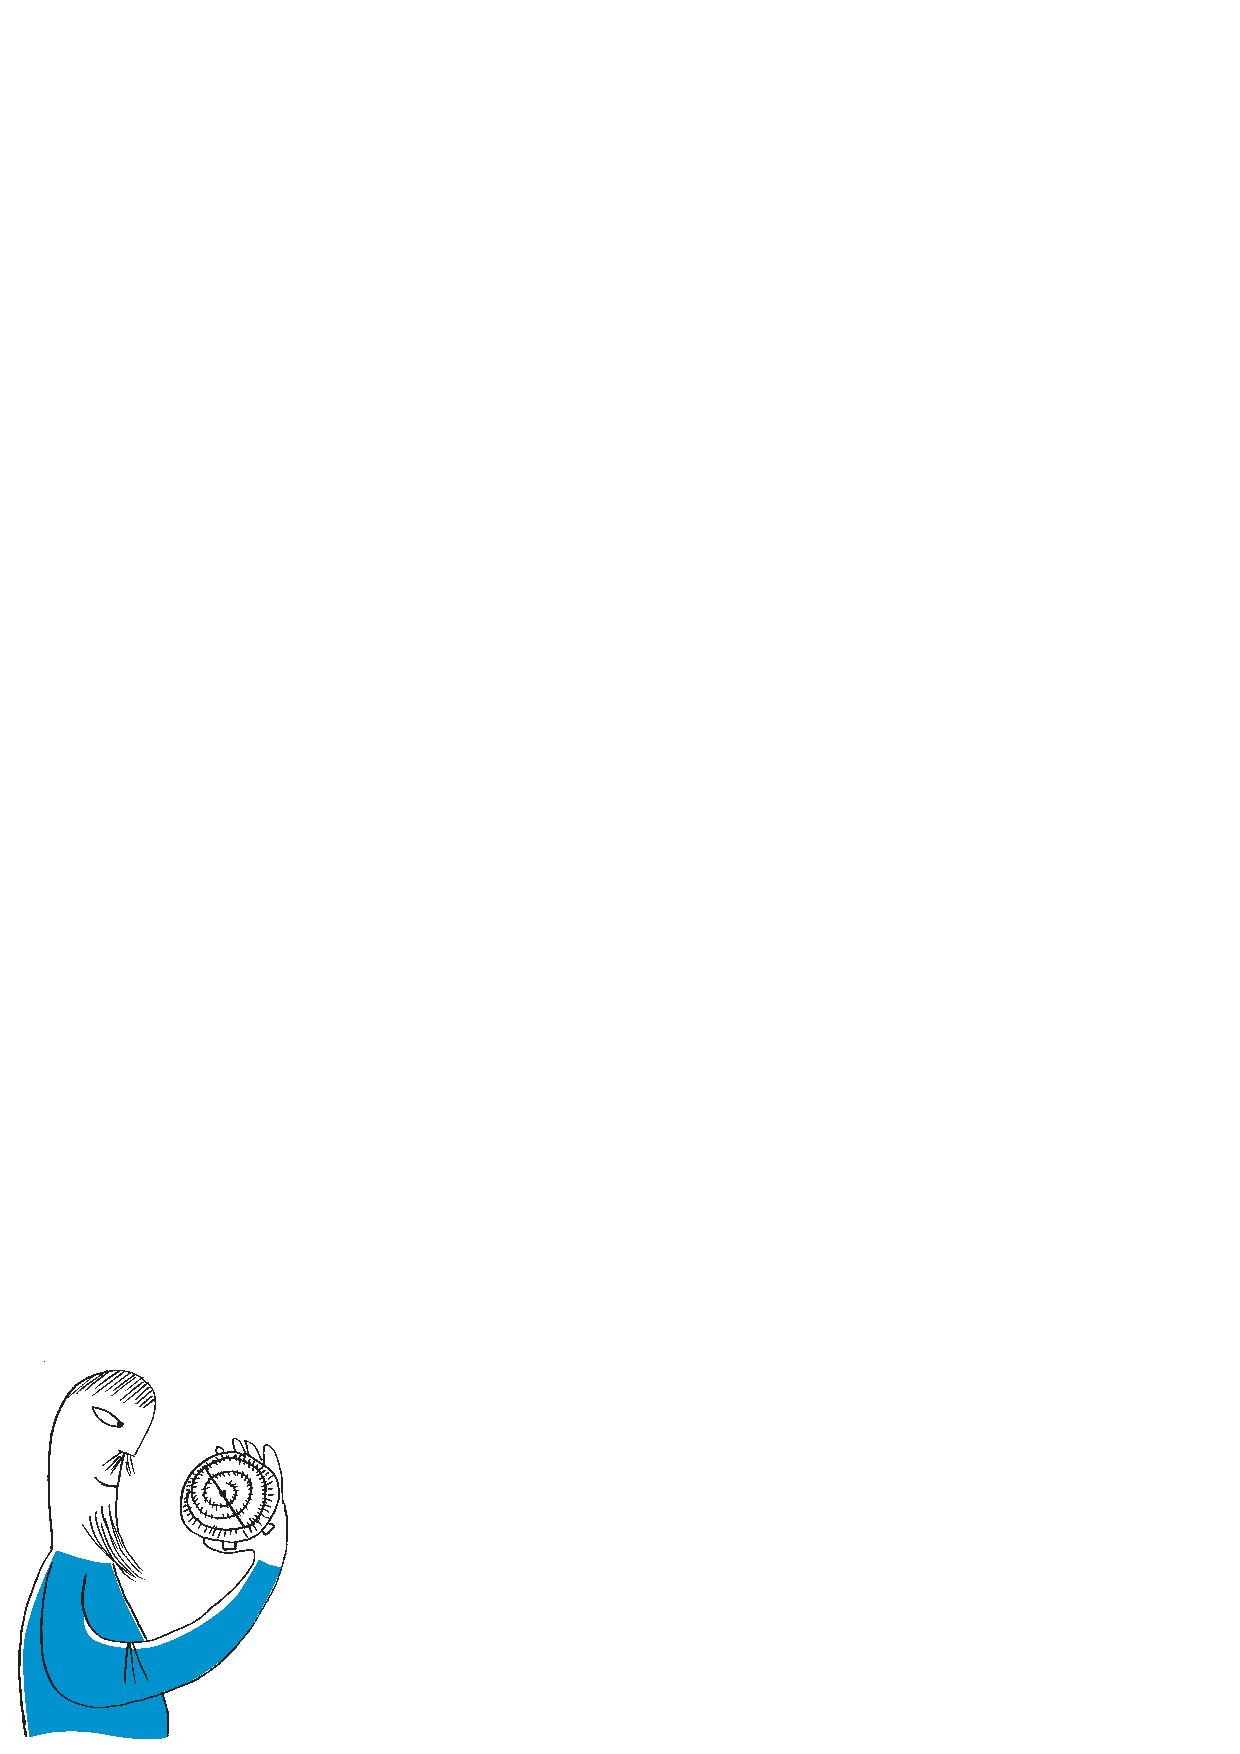
\includegraphics{art/202501_kol06}} \vskip-10pt

\setlength{\epigraphwidth}{0.5\textwidth}
\epigraph{
\emph{But I~do know one and one is two \\
And if this one could be with you \\
What a~wonderful world this would be}\vspace*{-3pt}
}{``Wonderful world'', Sam Cooke\vrule height10pt width0pt} 
%\end{szeroko}

  
  \renewcommand{\Zadania}[1][0pt]{%
    
\zadspis
\phantomsection\label{zadania}\noindent\setbox0=\hbox to70pt{
\includegraphics{kot}\hss}%
\copy0{\Magenta{\LARGE\bf Zadania}}}

\def\zadMat#1{%
  \textbf{M~#1.} \csuse{zadM-#1}%\\%
  %Rozwiązanie na str.~\pageref{rozM-#1}%
}
\def\zadFiz#1{%
  \textbf{F~#1.} \csuse{zadF-#1}%\\%
 % Rozwiązanie na str.~\pageref{rozF-#1}%
}

\vspace*{-6pt}
\begin{szeroko}
\Zadania\hfill
{\normalsize
\Magenta{\bf Rozwiązania na str.~\pageref{rozwiazania}}
}%
\end{szeroko}
\vspace*{6pt}
\begin{dwieszpalty}
\advance\rightskip by-1.3cm  \redaguje{Przygotował  Dominik BUREK}

\zadMat{1804}

\zadMat{1805}

\zadMat{1806}

\advance\rightskip by1.3cm 
\advance\leftskip by1.35cm 
\redaguje{Przygotował Andrzej MAJHOFER}

\zadFiz{1111}



\looseness1\zadFiz{1112}

\end{dwieszpalty}

